% =====================================================================
\section{Soldiers: Splines, Gait and Inverse Kinematics}\label{sec:soldiers}
\pipestrip{2}
The camp is manned by \nSoldiers{} soldiers (\code{objects/Soldier}, \code{scene/Gait}, \code{scene/Garrison}, \code{math/Spline}). They are friendly personnel with no damage model: blasts only make them duck, the UAVs never engage them (Section~\ref{sec:realcv}). Each soldier is a \code{Controllable} with a duty roster, routes planned on a site grid and a gait animated by forward and inverse kinematics; \texttt{F3} possesses one. Together they add \garrisonParts{} primitive parts to the scene.

\subsection{The figure as a hierarchy}
A soldier is \soldierParts{} leaves (\soldierPrims) under \soldierGroups{} joint groups, depth \soldierDepth{} (Figure~\ref{fig:soldiertree}). Every joint is a group node whose local rotation is a pose angle; limbs are capsules (a cylinder with two spheres), the rifle is held by arm IK or slung. The same $W=W_\text{parent}\,T\,R\,S$ chain as every other object places the parts (Section~\ref{sec:transform}); the exploded and axes views of Figure~\ref{fig:soldierviews} come from the generic explode and frame-axes passes.
\begin{figure}[h]
\centering
\begin{minipage}[c]{0.40\linewidth}\centering\resizebox{\linewidth}{!}{% generated by report/gen_tables.py from build/scene_export.json -- do not edit
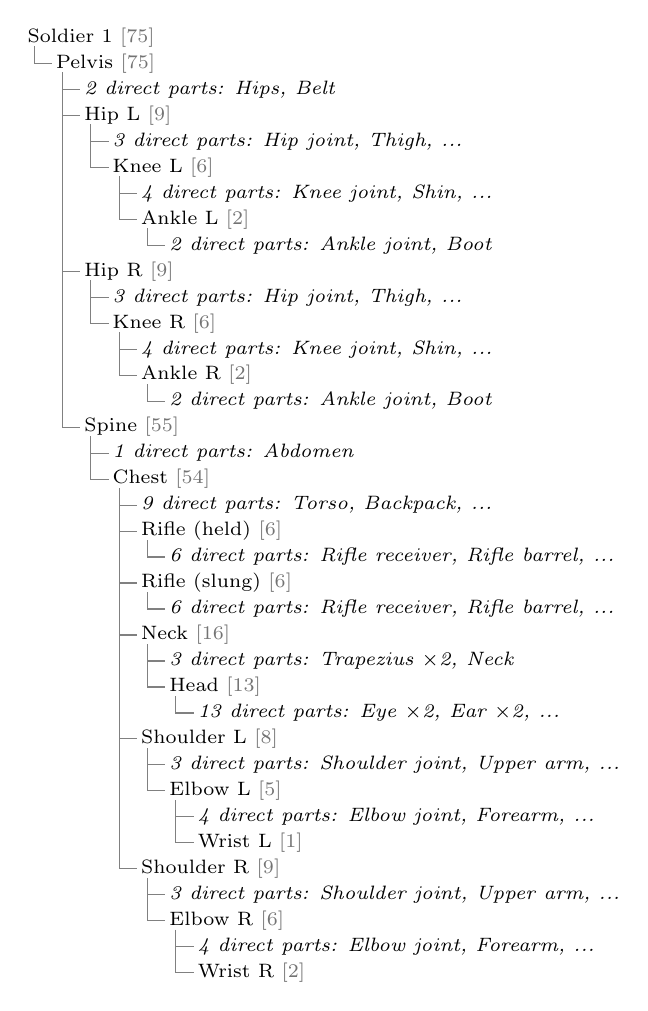
\begin{tikzpicture}[x=0.36cm,y=-0.33cm,font=\scriptsize]
\node[anchor=west,inner sep=0pt] (n0) at (0,0) {Soldier 1 \textcolor{black!55}{[75]}};
\node[anchor=west,inner sep=0pt] (n1) at (1,1) {Pelvis \textcolor{black!55}{[75]}};
\draw[black!50,thin] (0.25,0.35) |- (0.88,1);
\node[anchor=west,inner sep=0pt] (n2) at (2,2) {\textit{2 direct parts: Hips, Belt}};
\draw[black!50,thin] (1.25,1.35) |- (1.88,2);
\node[anchor=west,inner sep=0pt] (n3) at (2,3) {Hip L \textcolor{black!55}{[9]}};
\draw[black!50,thin] (1.25,1.35) |- (1.88,3);
\node[anchor=west,inner sep=0pt] (n4) at (3,4) {\textit{3 direct parts: Hip joint, Thigh, ...}};
\draw[black!50,thin] (2.25,3.35) |- (2.88,4);
\node[anchor=west,inner sep=0pt] (n5) at (3,5) {Knee L \textcolor{black!55}{[6]}};
\draw[black!50,thin] (2.25,3.35) |- (2.88,5);
\node[anchor=west,inner sep=0pt] (n6) at (4,6) {\textit{4 direct parts: Knee joint, Shin, ...}};
\draw[black!50,thin] (3.25,5.35) |- (3.88,6);
\node[anchor=west,inner sep=0pt] (n7) at (4,7) {Ankle L \textcolor{black!55}{[2]}};
\draw[black!50,thin] (3.25,5.35) |- (3.88,7);
\node[anchor=west,inner sep=0pt] (n8) at (5,8) {\textit{2 direct parts: Ankle joint, Boot}};
\draw[black!50,thin] (4.25,7.35) |- (4.88,8);
\node[anchor=west,inner sep=0pt] (n9) at (2,9) {Hip R \textcolor{black!55}{[9]}};
\draw[black!50,thin] (1.25,1.35) |- (1.88,9);
\node[anchor=west,inner sep=0pt] (n10) at (3,10) {\textit{3 direct parts: Hip joint, Thigh, ...}};
\draw[black!50,thin] (2.25,9.35) |- (2.88,10);
\node[anchor=west,inner sep=0pt] (n11) at (3,11) {Knee R \textcolor{black!55}{[6]}};
\draw[black!50,thin] (2.25,9.35) |- (2.88,11);
\node[anchor=west,inner sep=0pt] (n12) at (4,12) {\textit{4 direct parts: Knee joint, Shin, ...}};
\draw[black!50,thin] (3.25,11.35) |- (3.88,12);
\node[anchor=west,inner sep=0pt] (n13) at (4,13) {Ankle R \textcolor{black!55}{[2]}};
\draw[black!50,thin] (3.25,11.35) |- (3.88,13);
\node[anchor=west,inner sep=0pt] (n14) at (5,14) {\textit{2 direct parts: Ankle joint, Boot}};
\draw[black!50,thin] (4.25,13.35) |- (4.88,14);
\node[anchor=west,inner sep=0pt] (n15) at (2,15) {Spine \textcolor{black!55}{[55]}};
\draw[black!50,thin] (1.25,1.35) |- (1.88,15);
\node[anchor=west,inner sep=0pt] (n16) at (3,16) {\textit{1 direct parts: Abdomen}};
\draw[black!50,thin] (2.25,15.35) |- (2.88,16);
\node[anchor=west,inner sep=0pt] (n17) at (3,17) {Chest \textcolor{black!55}{[54]}};
\draw[black!50,thin] (2.25,15.35) |- (2.88,17);
\node[anchor=west,inner sep=0pt] (n18) at (4,18) {\textit{9 direct parts: Torso, Backpack, ...}};
\draw[black!50,thin] (3.25,17.35) |- (3.88,18);
\node[anchor=west,inner sep=0pt] (n19) at (4,19) {Rifle (held) \textcolor{black!55}{[6]}};
\draw[black!50,thin] (3.25,17.35) |- (3.88,19);
\node[anchor=west,inner sep=0pt] (n20) at (5,20) {\textit{6 direct parts: Rifle receiver, Rifle barrel, ...}};
\draw[black!50,thin] (4.25,19.35) |- (4.88,20);
\node[anchor=west,inner sep=0pt] (n21) at (4,21) {Rifle (slung) \textcolor{black!55}{[6]}};
\draw[black!50,thin] (3.25,17.35) |- (3.88,21);
\node[anchor=west,inner sep=0pt] (n22) at (5,22) {\textit{6 direct parts: Rifle receiver, Rifle barrel, ...}};
\draw[black!50,thin] (4.25,21.35) |- (4.88,22);
\node[anchor=west,inner sep=0pt] (n23) at (4,23) {Neck \textcolor{black!55}{[16]}};
\draw[black!50,thin] (3.25,17.35) |- (3.88,23);
\node[anchor=west,inner sep=0pt] (n24) at (5,24) {\textit{3 direct parts: Trapezius $\times$2, Neck}};
\draw[black!50,thin] (4.25,23.35) |- (4.88,24);
\node[anchor=west,inner sep=0pt] (n25) at (5,25) {Head \textcolor{black!55}{[13]}};
\draw[black!50,thin] (4.25,23.35) |- (4.88,25);
\node[anchor=west,inner sep=0pt] (n26) at (6,26) {\textit{13 direct parts: Eye $\times$2, Ear $\times$2, ...}};
\draw[black!50,thin] (5.25,25.35) |- (5.88,26);
\node[anchor=west,inner sep=0pt] (n27) at (4,27) {Shoulder L \textcolor{black!55}{[8]}};
\draw[black!50,thin] (3.25,17.35) |- (3.88,27);
\node[anchor=west,inner sep=0pt] (n28) at (5,28) {\textit{3 direct parts: Shoulder joint, Upper arm, ...}};
\draw[black!50,thin] (4.25,27.35) |- (4.88,28);
\node[anchor=west,inner sep=0pt] (n29) at (5,29) {Elbow L \textcolor{black!55}{[5]}};
\draw[black!50,thin] (4.25,27.35) |- (4.88,29);
\node[anchor=west,inner sep=0pt] (n30) at (6,30) {\textit{4 direct parts: Elbow joint, Forearm, ...}};
\draw[black!50,thin] (5.25,29.35) |- (5.88,30);
\node[anchor=west,inner sep=0pt] (n31) at (6,31) {Wrist L \textcolor{black!55}{[1]}};
\draw[black!50,thin] (5.25,29.35) |- (5.88,31);
\node[anchor=west,inner sep=0pt] (n32) at (4,32) {Shoulder R \textcolor{black!55}{[9]}};
\draw[black!50,thin] (3.25,17.35) |- (3.88,32);
\node[anchor=west,inner sep=0pt] (n33) at (5,33) {\textit{3 direct parts: Shoulder joint, Upper arm, ...}};
\draw[black!50,thin] (4.25,32.35) |- (4.88,33);
\node[anchor=west,inner sep=0pt] (n34) at (5,34) {Elbow R \textcolor{black!55}{[6]}};
\draw[black!50,thin] (4.25,32.35) |- (4.88,34);
\node[anchor=west,inner sep=0pt] (n35) at (6,35) {\textit{4 direct parts: Elbow joint, Forearm, ...}};
\draw[black!50,thin] (5.25,34.35) |- (5.88,35);
\node[anchor=west,inner sep=0pt] (n36) at (6,36) {Wrist R \textcolor{black!55}{[2]}};
\draw[black!50,thin] (5.25,34.35) |- (5.88,36);
\end{tikzpicture}
}\end{minipage}\hfill
\begin{minipage}[c]{0.58\linewidth}\centering
\picsix{soldier_closeup}{0.49\linewidth}\hfill\picsix{soldier_axes}{0.49\linewidth}\\[1mm]
\picsix{soldier_exploded}{0.49\linewidth}\hfill\picsix{soldier_possess_tp}{0.49\linewidth}
\end{minipage}
\caption{Left: node tree of soldier 1 (generated from the export; [n] = leaves below). Right: close-up, joint frames (\texttt{H}), primitive colours (\texttt{E}; the soldier roots are not yet in the explode list, so the parts stay assembled) and a possessed soldier in third person.}\label{fig:soldiertree}\label{fig:soldierviews}
\end{figure}

\subsection{Routes: centripetal Catmull--Rom splines}
\autofig{diagrams}{H3_catmull_rom}
A route through control points $P_0..P_n$ must pass through them, have a continuous tangent and no cusps or loops. A Catmull--Rom spline with knots $t_{i+1}=t_i+|P_{i+1}-P_i|^\alpha$ meets the first two for every $\alpha$; Yuksel et al.\ showed that only the \emph{centripetal} choice $\alpha=\tfrac12$ guarantees no cusp or self-intersection inside a segment. Each segment $P_1\to P_2$ is evaluated as a cubic Hermite curve in $u\in[0,1]$ with end tangents
\begin{equation}
\vect m_1=(t_2-t_1)\Bigl(\tfrac{P_1-P_0}{t_1-t_0}-\tfrac{P_2-P_0}{t_2-t_0}+\tfrac{P_2-P_1}{t_2-t_1}\Bigr),\qquad
\vect m_2=(t_2-t_1)\Bigl(\tfrac{P_2-P_1}{t_2-t_1}-\tfrac{P_3-P_1}{t_3-t_1}+\tfrac{P_3-P_2}{t_3-t_2}\Bigr),
\end{equation}
$\vect r(u)=h_{00}P_1+h_{10}\vect m_1+h_{01}P_2+h_{11}\vect m_2$ with the Hermite basis $h_{00}=2u^3-3u^2+1$, $h_{10}=u^3-2u^2+u$, $h_{01}=-2u^3+3u^2$, $h_{11}=u^3-u^2$. This equals the Barry--Goldman pyramid and is $C^1$ in the knot parameter. Open routes get mirrored phantom end points $2P_0-P_1$. The first and second derivatives come from the same basis, so the curvature is analytic:
\begin{equation}\kappa=\frac{|\vect r'\times\vect r''|}{|\vect r'|^3}\qquad\text{(independent of the parameterisation).}\end{equation}
\lstSplineSeg
\paragraph{Arc length.} Walking at a speed needs $\vect r(s)$ with $s$ in metres. Each segment is cut into 64 chords; their cumulative lengths form a monotone table and $s\mapsto t$ is a binary search plus a linear blend inside the chord (Listing~\ref{lst:ArcLen}). T200 checks interpolation, the joint kink, length and curvature errors (\tobs{T200}).
\lstArcLen

\subsection{Speed along a curve}
People slow down in tight turns. The soldier's speed limit is a function of the curvature,
\begin{equation}v_\kappa(s)=\max\bigl(0.25,\ v_\text{max}/(1+1.5\,\kappa(s))\bigr),\end{equation}
taken as a minimum over the next 0.5\,m. Braking is planned ahead: with a deceleration of $2.5$\,m/s$^2$ a speed $v$ can still reach $v_\kappa(s+a)$ after $a$ metres if $v\le\sqrt{v_\kappa(s+a)^2+2\cdot2.5\,a}$, so the target is the minimum of that bound over $a\in[0,2]$\,m, and $\sqrt{2\cdot1.2\,d}+0.15$ before a stop $d$ metres ahead. The speed approaches the target at $+1.6$/$-4$\,m/s$^2$ and is clamped again at the end of the step because $\kappa$ is only piecewise continuous on a $C^1$ curve (T213: \tobs{T213}).
\lstSpeedLaw

\subsection{The site planner: A*, string pulling, spline}
Routes between camp sites are planned, not drawn. \code{SitePlanner} rasterises the camp onto $72\times72$ cells of 1\,m. Every static part that reaches into the body band (0.15--1.8\,m above the ground) contributes its exact oriented plan footprint (the convex hull of the projected unit primitive under its world matrix); fences, the trench and the HESCO ring are added as segments. A cell is free when its centre keeps 0.40\,m from every footprint. Then:
\begin{enumerate}
\item \textbf{A*} on the 8-connected free cells with the octile heuristic $h=\max(\Delta i,\Delta j)+(\sqrt2-1)\min(\Delta i,\Delta j)$, which is the exact distance on an obstacle-free 8-grid and therefore admissible and consistent; diagonal moves may not cut a blocked corner (Listing~\ref{lst:AStar}).
\item \textbf{String pulling}: from each kept point, the farthest later grid point whose straight segment keeps the clearance (sampled every 0.1\,m) is kept; the staircase of grid steps collapses to a few corners (Listing~\ref{lst:StringPull}).
\item \textbf{Spline} through the kept points, validated every 0.1\,m against a body clearance of 0.28\,m. Where a sample fails, the grid points around it are re-inserted; in the limit the spline passes through every cell centre, whose edges are clear by construction.
\end{enumerate}
The bunker is reached by a hand-authored leg (ramp, blast doors, tunnel, rooms) with floor heights from the walk space. For the \nRoutes{} routes of the roster ($\routeTotal$\,m in total) the smallest clearance is \routeMinClear\,m (Table~\ref{tab:routes}; T205: \tobs{T205}).
\begin{figure}[h]
\centering
\begin{subfigure}{0.495\linewidth}\picsix{plan_routes}{\linewidth}\caption{Tactical map (\texttt{M}): soldier splines and rover via chains}\end{subfigure}
\begin{subfigure}{0.495\linewidth}\picsix{day_patrol_spline}{\linewidth}\caption{Spline routes drawn over the camp by day}\end{subfigure}
\caption{Planned routes (captures).}\label{fig:routes}
\end{figure}
\lstAStar
\lstStringPull
\begin{table}[h]
\centering\scriptsize
\caption{Roster routes (generated from \code{v6.garrison.routes}).}\label{tab:routes}
\tabRoutes
\end{table}

\subsection{Gait: forward kinematics driven by a foot trajectory}
\autofig{diagrams}{H4_gait_cycle}
A walk cycle is defined by where the feet must be, not by key frames. Leg 0 touches down at phase 0, leg 1 at 0.5; the stance lasts the duty fraction $\beta$ of the cycle. With the stride $L$ the ankle position relative to the hip is
\begin{equation}
x_\text{stance}(\sigma)=x_f-(x_f-x_b)\,\sigma,\qquad
x_\text{swing}(\sigma)=x_b+(x_f-x_b)\Bigl(\sigma-\frac{\sin2\pi\sigma}{2\pi}\Bigr),\qquad y_\text{swing}\mathrel{+}=\ell\sin\pi\sigma,
\end{equation}
$x_{f,b}=\pm\tfrac12L\beta-r$ ($\sigma$ = fraction of the stance or swing done, $r$ a push-off offset). In stance the ankle moves backwards at exactly the body speed, so it stands still in the world; the swing is a cycloid, whose velocity relative to the body is zero at lift-off and touch-down (no foot skating). The pelvis bobs twice per cycle, the trunk counter-rotates and each arm swings against its leg (T204: \tobs{T204}). Walk and run differ only in parameters (Table~\ref{tab:gait}). The joint angles that place the ankle there come from IK.
\begin{table}[h]
\centering\small
\caption{Gait parameters (generated from \code{v6.garrison.gait}).}\label{tab:gait}
\tabGait
\end{table}
\lstFootPath

\subsection{Two-link inverse kinematics}
\autofig{diagrams}{H5_two_link_ik}
Thigh $L_1=\gaitThigh$\,m and shin $L_2=\gaitShin$\,m form a triangle with the hip--ankle distance $d=|(x,y)|$, clamped to $[\,|L_1-L_2|,\,L_1+L_2]$. The law of cosines gives
\begin{equation}
\theta_k=\pi-\arccos\frac{L_1^2+L_2^2-d^2}{2L_1L_2},\qquad
\theta_h=\operatorname{atan2}(x,-y)+\arccos\frac{L_1^2+d^2-L_2^2}{2L_1d},
\end{equation}
knee bend $\theta_k$ (0 = straight) and thigh angle $\theta_h$ from the vertical, with the knee in front of the hip--ankle line. Forward kinematics, $x=L_1\sin\theta_h+L_2\sin(\theta_h-\theta_k)$, $y=-L_1\cos\theta_h-L_2\cos(\theta_h-\theta_k)$, closes the loop: T203 measures $|FK(IK(\vect p))-\vect p|$ (\tobs{T203}). In the scene the stance foot's world point is \emph{locked} at touch-down and the IK solves for that point every frame, so the foot does not slide on slopes or in turns (T202: \tobs{T202}). The ankle keeps the sole level (ankle $=\theta_k-\theta_h$) and pivots on the toe at push-off.
\lstLegIK

\paragraph{Arms: two-bone IK with a pole vector (v7).} Armed soldiers hold the rifle with both hands. For a shoulder $S$, a hand target $T$ on the rifle grip and a pole direction $\vect p$ (where the elbow should point), the solver in the chest frame takes $\hat{\vect e}=(T-S)/d$, the pole's part perpendicular to it $\hat{\vect p}_\perp$ and the angle $A$ at the shoulder from the law of cosines; the upper arm is $\hat{\vect u}=\hat{\vect e}\cos A+\hat{\vect p}_\perp\sin A$, the elbow $S+\ell_u\hat{\vect u}$, the forearm $\hat{\vect v}$ points from the elbow to $T$ and the elbow bend is $\arccos(\hat{\vect u}\cdot\hat{\vect v})$. The shoulder rotation is the basis $(\vect x,\vect y,\vect z)=(\vect y\times\vect z,\ -\hat{\vect u},\ \text{forearm direction}\perp\hat{\vect u})$, converted to the rig's Euler order $M=R_yR_xR_z$ by $\text{pitch}=\arcsin(-z_y)$, $\text{yaw}=\operatorname{atan2}(z_x,z_z)$, $\text{roll}=\operatorname{atan2}(x_y,y_y)$.
\lstArmIK

\subsection{Roster, shifts and behaviour}
Each soldier has a duty with a day and a night program (Table~\ref{tab:roster}). The day shift runs from \shiftStart{} to \shiftEnd, matching the DayBreak and Dusk crossings of Section~\ref{sec:daycycle}. At dusk the departures are staggered; soldiers going below walk the ramp, wait at closed blast doors, pass the tunnel and sit down in the bunk room or the mess (T207: \tobs{T207}). A soldier's state machine cycles through Idle, Guard, Work, Sit, Walk, Run, Wait, Duck, Crouch and Wave; work loops play at the vehicles (mechanic's wrench at the tank deck and the helicopter, logistics carrying crates; T210). Walkers yield or pass on the side away from each other with a validated lateral offset (T214: \tobs{T214}). In the thermal view a soldier is warm but never engine-hot: face and hands 0.82, torso 0.70, below the 0.90 core of a rover (T209), and each soldier carries a friendly radius of \soldierFriendly\,m for the squad (Section~\ref{sec:realcv}).
\begin{table}[h]
\centering\scriptsize
\caption{Duty roster (generated from \code{v6.garrison.soldiers}).}\label{tab:roster}
\tabRoster
\end{table}
\begin{figure}[h]
\centering
\begin{subfigure}{0.495\linewidth}\picsix{day_mechanic}{\linewidth}\caption{Mechanic at the tank (wrench)}\end{subfigure}
\begin{subfigure}{0.495\linewidth}\picsix{day_logistics}{\linewidth}\caption{Logistics carrying a crate}\end{subfigure}\\[1mm]
\begin{subfigure}{0.495\linewidth}\picsix{dusk_shift_change}{\linewidth}\caption{Dusk: shift-change banner}\end{subfigure}
\begin{subfigure}{0.495\linewidth}\picsix{bunker_offduty}{\linewidth}\caption{Off duty in the bunk room (night)}\end{subfigure}\\[1mm]
\begin{subfigure}{0.495\linewidth}\picsix{soldier_possess_fp}{\linewidth}\caption{Possessed soldier, first person}\end{subfigure}
\caption{Duties over the day (captures, RTX\,4070).}\label{fig:duties}
\end{figure}
\sheetfig{sheet_soldiers}
